\documentclass[conference]{IEEEtran}

\usepackage{amsmath,amssymb}
\usepackage{booktabs}
\usepackage{graphicx}
\usepackage{xcolor}
\usepackage{url}
\usepackage[hidelinks,pdftitle={Do Visual Grounding Decoders Need Feed-Forward Networks?},pdfauthor={Anonymous}]{hyperref}

\graphicspath{{../figures/}{./}}

\title{Do Visual Grounding Decoders Need Feed-Forward Networks?}
\author{Anonymous Submission}

\begin{document}
\maketitle

\begin{abstract}
Do feed-forward networks (FFNs) in visual grounding decoders remain necessary after a pretrained vision-language model has contextualized the image and language? We compare a four-block attention-only decoder (A4), a matched attention-plus-FFN decoder (S4), and an eight-block attention-only parameter control (A8) over frozen VLM features. A4 matches S4 on RefCOCOg and is 0.79 percentage points better on Ref-Adv-s. FineCops-Ref exposes a small A4 deficit of 0.52 points at IoU@0.5; A8 recovers it. A4 uses 44.4\% fewer trainable decoder parameters and 10.1\% lower cached-decoder latency. The evidence supports a bounded conclusion: FFNs are often dispensable in this small trainable grounding decoder, while the frozen VLM and its pretrained FFNs remain unchanged.
\end{abstract}

\section{Introduction}
Visual grounding maps an image and a referring expression to one target box. Standard Transformer grounding heads combine attention with a token-wise feed-forward network (FFN) in each block. This is a sensible default when the model must construct representations from raw inputs.

Our question is narrower. If a frozen vision-language model (VLM) already provides contextual image patches and text states, does a small task decoder still need its FFN residuals? We delete only those residuals while keeping the frozen features, projections, attention, readout, loss, optimizer, and box conversion fixed.

We compare A4, a four-block FFN-free decoder, with S4, the identical four-block decoder with FFNs. A8 doubles attention-only depth to approximately match S4's trainable parameter count. This separates a fixed-depth deletion test from a capacity-reallocation test.

The study asks three questions: (1) does A4 retain standard grounding? (2) does a released or official difficulty variable expose an FFN advantage? and (3) can additional attention depth recover a fixed-depth gap?

The answer is mixed. A4 retains standard and adversarial grounding. FineCops-Ref shows a small fixed-depth compositional gap, and A8 recovers the overall difference. No evaluated difficulty scale shows a monotonic A4 failure boundary.

\begin{figure}[t]
  \centering
  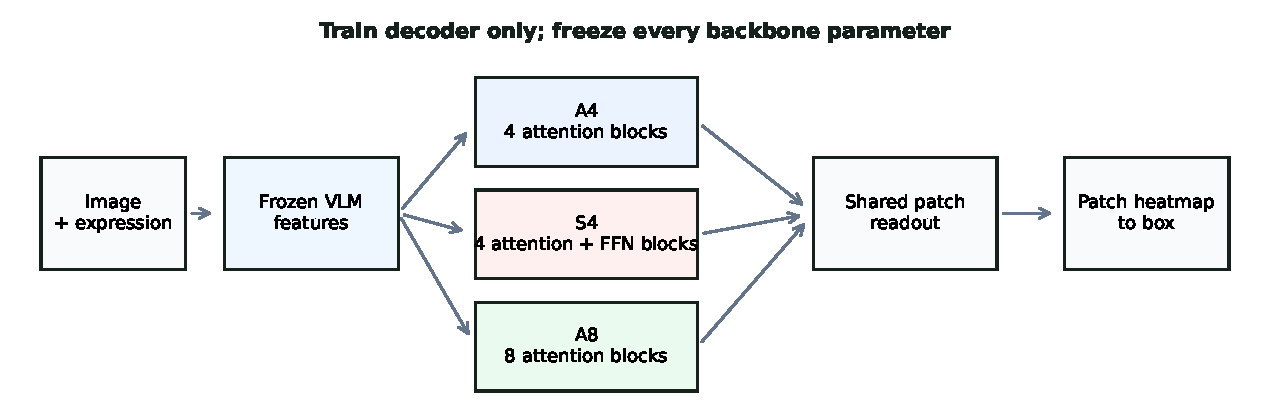
\includegraphics[width=\columnwidth]{generated-method-overview.pdf}
  \caption{The frozen VLM, projections, readout, supervision, and box conversion are shared. Only decoder capacity allocation changes.}
  \label{fig:method}
\end{figure}

\section{Method}
\subsection{Frozen representation and decoder}
The primary frozen backbone is SigLIP 2 Base/16 at 384 pixels. It yields 576 image tokens on a $24\times24$ grid and contextual text states. Linear projections map both streams to width 256.

A learned query alternates text and image cross-attention. S4 applies a pre-normalized GELU FFN after each attention pair. A4 omits these residuals. A8 uses eight attention-only blocks and has approximately the same trainable parameter count as S4.

The final query scores the 576 image patches. A softmax produces a patch distribution, trained against the target box's normalized patch-overlap distribution. A deterministic mass-to-box rule converts the heatmap to one box. There is no coordinate-regression MLP, segmentation refinement, auxiliary loss, multi-query head, or backbone adaptation.

\subsection{Controlled comparison}
The heatmap mass threshold $\tau=0.8$ is selected once on RefCOCOg validation and frozen before held-out evaluation. All variants share data order, optimizer, learning rate, training budget, and evaluation code.

For three-seed comparisons, model predictions are paired per example. We use 10,000 image-clustered bootstrap replicates so expressions from one image are not treated as independent images. Positive differences favor A4.

\section{Experimental Setup}
\subsection{Benchmarks}
RefCOCOg UMD is the primary three-seed study. It supplies standard referring expressions and modality-shuffle controls. RefCOCO UNC is a seed-0 classic-dataset check.

Ref-Adv-s is an evaluation-only stress test with released negation, expression-length, and distractor metadata. FineCops-Ref is the controlled compositional test; we use its official positive-test split, levels, and tuple types without inventing post-hoc semantic labels.

We also report a descriptive one-seed frozen CLIP L/14@336 control. It preserves the 24-by-24 patch geometry while changing the representation family.

\subsection{Metrics and efficiency}
The primary metric is the fraction of examples with IoU at least 0.5 (IoU@0.5). We report percentage-point differences with bootstrap intervals when available. Efficiency uses the same frozen SigLIP2 features and measures cached-decoder latency separately from full-pipeline latency.

\section{Results}
\subsection{Standard and adversarial grounding}
On RefCOCOg direct expressions, A4 is 0.26 points above S4 (90\% CI $[-0.33,+0.84]$). The direct-retention gate passes, while the planned direct-versus-logical interaction is not confirmed.

On Ref-Adv-s, A4 is 0.79 points above S4 (95\% CI $[+0.06,+1.52]$). Negation, expression length, and distractor-count slices do not show a monotonic A4 loss. Image and text shuffles sharply reduce both A4 and S4, indicating that both modalities matter.

\begin{table}[t]
\centering
\caption{Primary paired differences at IoU@0.5. Positive values favor A4.}
\label{tab:results}
\small
\begin{tabular}{lrr}
\toprule
Evaluation & A4--S4 (pp) & Interval \\
\midrule
RefCOCOg direct & +0.26 & 90\% CI $[-0.33,+0.84]$ \\
Ref-Adv-s & +0.79 & 95\% CI $[+0.06,+1.52]$ \\
FineCops-Ref & -0.52 & 95\% CI $[-0.95,-0.12]$ \\
FineCops A8--S4 & +0.26 & paired estimate \\
CLIP control & +0.18 & one seed \\
\bottomrule
\end{tabular}
\end{table}

\subsection{Controlled composition}
FineCops-Ref reveals the only clear overall fixed-depth deficit. A4 is 0.52 points below S4 (95\% CI $[-0.95,-0.12]$) over 9,605 positive-test examples.

The deficit is similar at official levels 1 and 2. Level 3 slightly favors A4 but is imprecise. Tuple-type rows are descriptive and do not establish that more relations require more FFN computation.

\subsection{Capacity reallocation}
A8 is 0.26 points above S4 on FineCops overall. Since A8 is parameter-matched rather than compute-matched, this result supports attention capacity as a substitute at the measured scale. It does not prove that FFNs never provide a distinct function.

\begin{figure}[t]
  \centering
  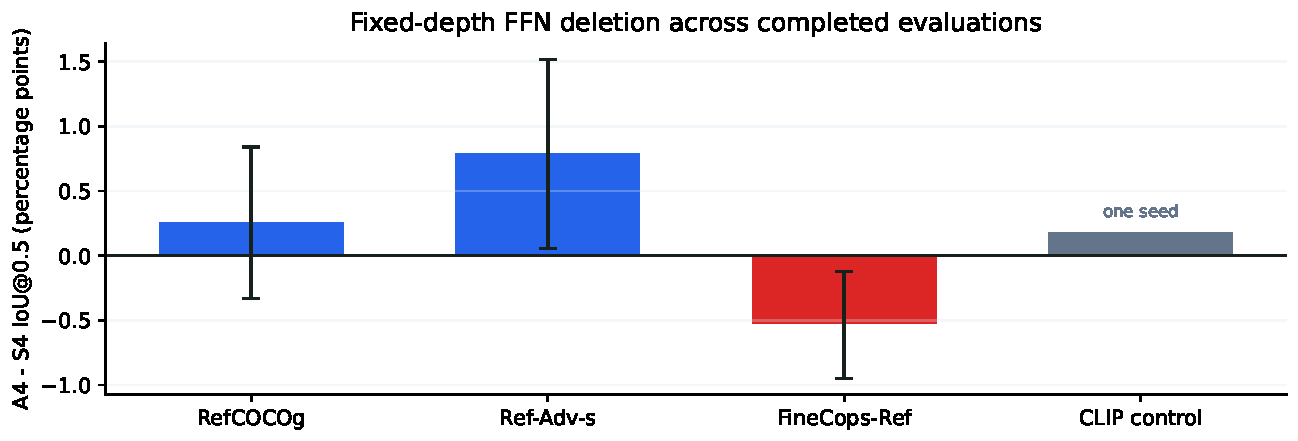
\includegraphics[width=\columnwidth]{generated-evidence-overview.pdf}
  \caption{A4--S4 differences across completed evaluations. FineCops-Ref is the only overall comparison with a clear fixed-depth A4 deficit.}
  \label{fig:evidence}
\end{figure}

\subsection{Efficiency and transfer}
A4 has 2.64M trainable decoder parameters versus 4.74M for S4, a 44.4\% reduction. Cached-decoder latency falls from 7.46 ms to 6.71 ms, a 10.1\% reduction. Full-pipeline latency changes by only 0.4\% because the frozen VLM dominates.

The frozen CLIP control has A4--S4 = +0.18 points on RefCOCOg. It is one seed and descriptive only, so it supports directional transfer rather than a new significance claim.

\section{Related Work and Limitations}
MDETR and Grounding DINO retain standard Transformer FFNs in multimodal detection and grounding stacks \cite{kamath2021mdetr,liu2024groundingdino}. Frozen-CLIP region scoring and attention-based frozen-LVLM grounding show that pretrained representations contain useful localization signals \cite{subramanian2022reclip,kang2025heads,wu2025flmm}. Our intervention isolates a matched trainable decoder FFN comparison.

Attention-only Transformer studies motivate reallocating FFN capacity into depth \cite{ndubuaku2026attention}. Synthetic compositional grounding work also shows that depth and composition interact \cite{sikarwar2022groundcompose}. We test the corresponding capacity question on real images over frozen VLM features.

The claim is bounded to a one-query box-grounding decoder. The backbone is frozen and retains its pretrained FFNs. The output is one box from a 24-by-24 patch heatmap, not segmentation or multi-object detection. FineCops level-3 and small tuple slices are noisy. RefCOCO UNC and CLIP are descriptive replications.

\section{Conclusion}
In this frozen-VLM grounding decoder, fixed-depth FFN removal preserves standard and adversarial performance. A small compositional deficit appears on FineCops-Ref, and additional attention depth recovers it at a similar parameter budget.

The supported conclusion is architectural and narrow: when a strong frozen VLM has already contextualized visual and linguistic information, attention-only decoder capacity can often replace FFN capacity for single-query grounding.

\section*{AI-use disclosure}
AI tools assisted with language editing and software organization. The authors verified all methods, numbers, citations, figures, and conclusions.

\bibliographystyle{IEEEtran}
\bibliography{references}

\end{document}
